% !TEX program = tectonic
% Standalone English analysis. Compile from the repository root:
% tectonic --outdir docs/gae_reward_support/build docs/gae_reward_support/gae_reward_support_analysis.tex
\documentclass[11pt,a4paper]{article}
\usepackage[margin=2.3cm]{geometry}
\usepackage{amsmath,amssymb,bm,booktabs,array}
\usepackage{microtype}
\usepackage{xcolor}
\usepackage{tikz,pgfplots}
\pgfplotsset{compat=1.18}
\usetikzlibrary{arrows.meta}
\usepackage[colorlinks=true,linkcolor=blue!45!black,citecolor=blue!45!black,urlcolor=blue!60!black]{hyperref}
\usepackage{fancyhdr}
\setlength{\headheight}{14pt}
\pagestyle{fancy}\fancyhf{}
\fancyhead[L]{\small Reward Support and Critic Error in GAE}
\fancyfoot[C]{\thepage}
\setlength{\parskip}{0.35em}
\setlength{\parindent}{0pt}
\numberwithin{equation}{section}
\newcommand{\E}{\mathbb E}
\newcommand{\ind}{\mathbf 1}
\newcommand{\Var}{\operatorname{Var}}
\newcommand{\clip}{\operatorname{clip}}
\title{Reward Support Across Episode Positions:\\Exact Counts and Their Effect on GAE Critic Targets}
\author{Technical analysis for the tokamak control experiments}
\date{October 26, 2026}
\begin{document}
\maketitle
\begin{abstract}
A fixed-length rollout generally ends at a different position in each episode.
Consequently, advantages associated with different episode positions use different
numbers of observed rewards. We derive the exact cumulative support count $C_t$,
its periodic structure, and its relation to critic-target error. For the example
$M=500$, $N=256$, and $m=64$, the first position uses 130 rewards per target on
average, whereas the final position uses one. Under a controlled endpoint-error
perturbation, their average sensitivity coefficients are approximately 0.0651 and
0.995, respectively. All results assume \textbf{correct bootstrapping at artificial
episode time limits}. The analysis separates reward support, sample count, target
bias, and state coverage so that the effect can be quantified without treating
these different quantities as interchangeable.
\end{abstract}

\section{Sampling convention and the quantities being counted}
The sampling convention is the one illustrated by Figure 14.1 of the accompanying
\emph{Tokamak Plasma Simulator Guide}: rollout windows continue across resets,
while GAE recursion stops at both rollout boundaries and episode boundaries.
The derivation here is self-contained and does not require that figure.

Consider one environment. It produces $m$ episodes of exactly $M$ action steps
each, with no early failures. Rollouts contain $N$ transitions. The first rollout
starts at the first transition of the first episode. Episode $j$ is indexed by
$j=1,\ldots,m$, and position within an episode by $t=1,\ldots,M$.
At position $t$, the environment starts in $s_{j,t}$, takes $a_{j,t}$, receives
$r_{j,t}$, and reaches $s_{j,t+1}$.

An artificial time limit resets the environment after transition $M$ but does
not make the underlying control task terminal. Its final state is used for
bootstrap; rewards from the reset episode are never appended to the old episode's
GAE. A final partial rollout is assumed to be processed, or sampling is continued
until the containing rollout is complete. Discarding an incomplete final rollout
would require excluding the discarded samples from the counts below.

\begin{table}[htbp]\centering
\caption{Definitions. Counts include the current transition's reward.}
\begin{tabular}{@{}lp{11.4cm}@{}}\toprule
Symbol & Meaning \\\midrule
$m$ & Number of complete episodes from one environment. \\
$M$ & Actual episode length in transitions, not merely a configured maximum. \\
$N$ & Rollout length per environment. \\
$K_{j,t}$ & Number of rewards available to the GAE fragment starting at $(j,t)$. \\
$C_t$ & Sum of those support lengths over all $m$ episodes. \\
$\bar K_t=C_t/m$ & Average number of available rewards per target at position $t$. \\
$\gamma,\lambda$ & Discount and GAE trace parameters; $q=\gamma\lambda$. \\
\bottomrule\end{tabular}
\end{table}

There are $m$ training samples at every position $t$, regardless of $C_t$.
$C_t$ counts reward occurrences supporting these targets, not independent samples
and not additional simulator calls. Counts for different positions can reuse the
same rewards. A bootstrap value is a prediction and is not counted as an observed
reward. For $0<\gamma\lambda<1$, every available reward has a nonzero coefficient;
when $\lambda=0$, only the current reward contributes despite the larger available
support.

\section{Exact reward-support count}
\subsection{One sample}
The zero-based global transition index of $(j,t)$ is
\begin{equation}
 g_{j,t}=(j-1)M+t-1.
\end{equation}
The number of transitions remaining in its rollout, including the current one, is
\begin{equation}
 B_{j,t}=N-(g_{j,t}\bmod N).
\end{equation}
The number remaining in its episode is $R_t=M-t+1$. Therefore,
\begin{equation}\label{eq:K}
 \boxed{K_{j,t}=\min\left\{M-t+1,\;
 N-\bigl(((j-1)M+t-1)\bmod N\bigr)\right\}.}
\end{equation}
The actual rewards used are $r_{j,t},\ldots,r_{j,t+K_{j,t}-1}$.
Both boundaries matter: continuing to fill a rollout after reset does not extend
the preceding episode's reward support.


Figure~\ref{fig:support-intervals} makes the endpoints of these counts explicit.
Let $a_j=(j-1)M$ be the episode-start index and
$b_{j,t}=N\lfloor g_{j,t}/N\rfloor$ the containing rollout's start index.
The episode occupies $[a_j,a_j+M)$ and the rollout occupies
$[b_{j,t},b_{j,t}+N)$. Their common right endpoint for this target is
$h_{j,t}=\min(a_j+M,b_{j,t}+N)$, so $K_{j,t}=h_{j,t}-g_{j,t}$.
These are half-open intervals of \emph{transition indices}: the endpoint is
where a bootstrap state is available, not an extra observed reward.

\clearpage
\begin{figure}[p]
\centering
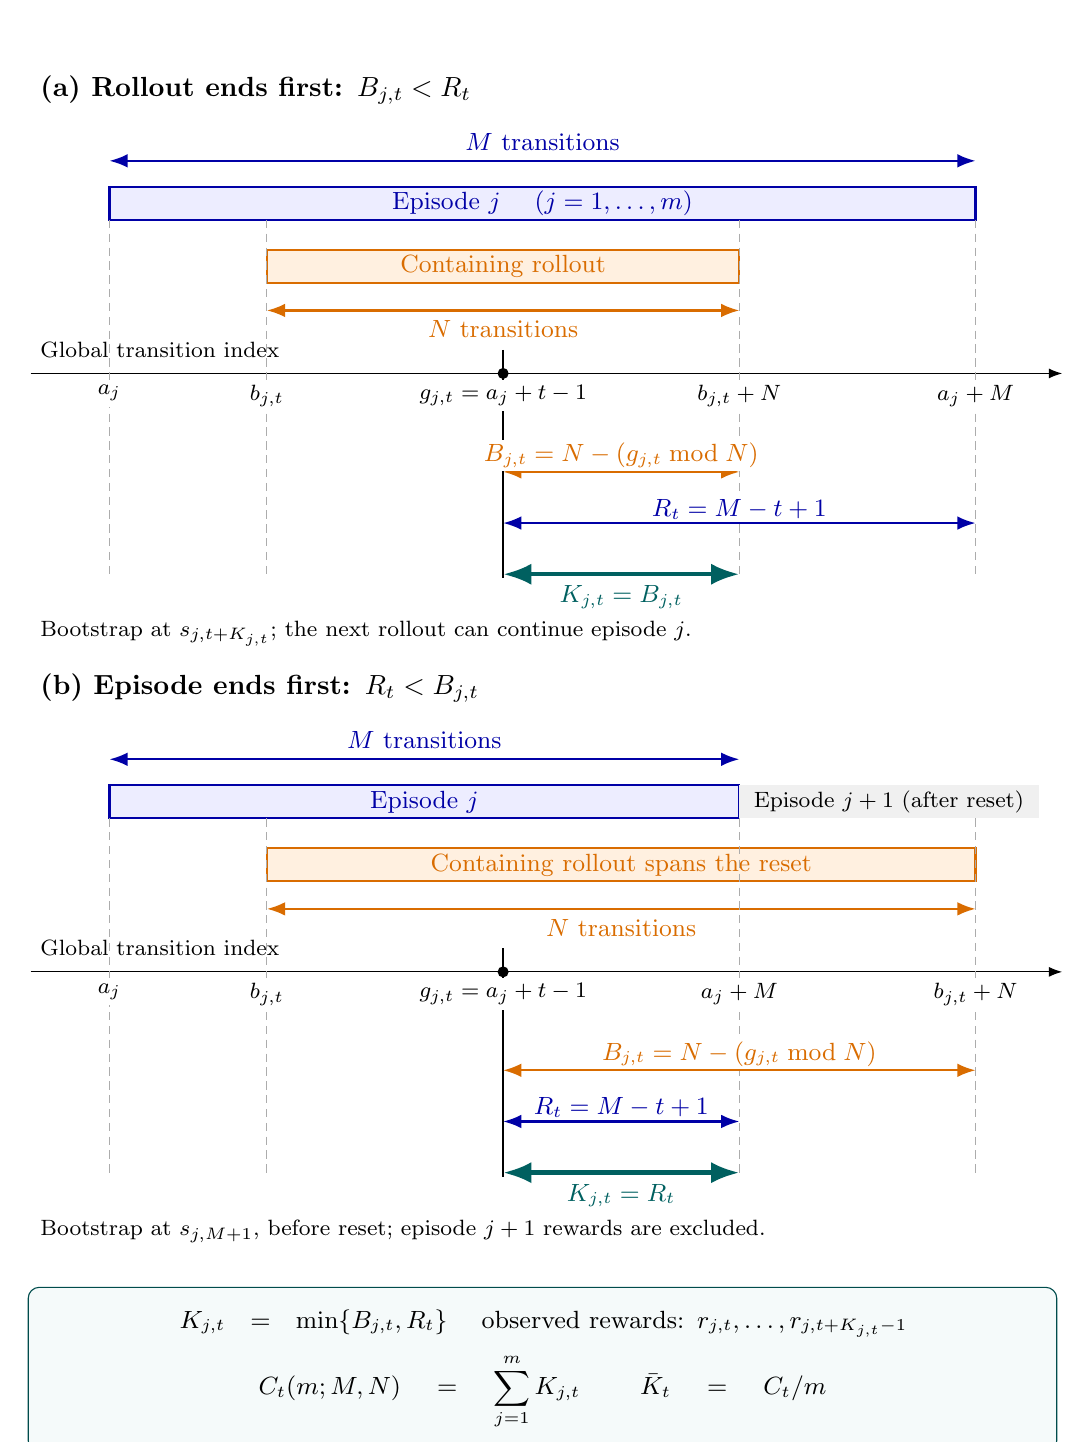
\begin{tikzpicture}[x=1cm,y=1cm,font=\small,
 measure/.style={<->,>=Latex,thick},
 guide/.style={densely dashed,gray!65},
 ep/.style={blue!65!black},roll/.style={orange!85!black},
 support/.style={teal!75!black}]
% Panel A: rollout boundary first.
\node[anchor=west,font=\bfseries] at (0,1.65)
 {(a) Rollout ends first: $B_{j,t}<R_t$};
\fill[blue!7] (1,0) rectangle (12,.42);
\draw[ep,thick] (1,0) rectangle (12,.42);
\node[ep] at (6.5,.21) {Episode $j$ \quad ($j=1,\ldots,m$)};
\draw[measure,ep] (1,.75)--node[above] {$M$ transitions}(12,.75);
\fill[orange!12] (3,-.8) rectangle (9,-.38);
\draw[roll,thick] (3,-.8) rectangle (9,-.38);
\node[roll] at (6,-.59) {Containing rollout};
\draw[measure,roll] (3,-1.15)--node[below] {$N$ transitions}(9,-1.15);
\draw[->,>=Latex] (0,-1.95)--(13.1,-1.95);
\foreach \x in {1,3,9,12} {\draw[guide] (\x,0)--(\x,-4.55);}
\draw[black,thick] (6,-1.65)--(6,-4.55);
\fill (6,-1.95) circle (2pt);
\node[anchor=west,font=\footnotesize] at (0,-1.65) {Global transition index};
\node[below=2pt,font=\footnotesize,fill=white,inner sep=2pt] at (1,-1.95) {$a_j$};
\node[below=2pt,font=\footnotesize,fill=white,inner sep=2pt] at (3,-1.95) {$b_{j,t}$};
\node[below=2pt,font=\footnotesize,fill=white,inner sep=2pt] at (6,-1.95) {$g_{j,t}=a_j+t-1$};
\node[below=2pt,font=\footnotesize,fill=white,inner sep=2pt] at (9,-1.95) {$b_{j,t}+N$};
\node[below=2pt,font=\footnotesize,fill=white,inner sep=2pt] at (12,-1.95) {$a_j+M$};
\draw[measure,roll] (6,-3.2)--node[above,fill=white,inner sep=1pt]
 {$B_{j,t}=N-(g_{j,t}\bmod N)$}(9,-3.2);
\draw[measure,ep] (6,-3.85)--node[above,fill=white,inner sep=1pt]
 {$R_t=M-t+1$}(12,-3.85);
\draw[measure,support,line width=1.6pt] (6,-4.5)--node[below]
 {$K_{j,t}=B_{j,t}$}(9,-4.5);
\node[anchor=west,align=left,font=\footnotesize] at (0,-5.25)
 {Bootstrap at $s_{j,t+K_{j,t}}$; the next rollout can continue episode $j$.};
% Panel B: episode boundary first.
\begin{scope}[yshift=-7.6cm]
\node[anchor=west,font=\bfseries] at (0,1.65)
 {(b) Episode ends first: $R_t<B_{j,t}$};
\fill[blue!7] (1,0) rectangle (9,.42);
\draw[ep,thick] (1,0) rectangle (9,.42);
\node[ep] at (5,.21) {Episode $j$};
\fill[gray!12] (9,0) rectangle (12.8,.42);
\node[font=\footnotesize] at (10.9,.21) {Episode $j+1$ (after reset)};
\draw[measure,ep] (1,.75)--node[above] {$M$ transitions}(9,.75);
\fill[orange!12] (3,-.8) rectangle (12,-.38);
\draw[roll,thick] (3,-.8) rectangle (12,-.38);
\node[roll] at (7.5,-.59) {Containing rollout spans the reset};
\draw[measure,roll] (3,-1.15)--node[below] {$N$ transitions}(12,-1.15);
\draw[->,>=Latex] (0,-1.95)--(13.1,-1.95);
\foreach \x in {1,3,9,12} {\draw[guide] (\x,0)--(\x,-4.55);}
\draw[black,thick] (6,-1.65)--(6,-4.55);
\fill (6,-1.95) circle (2pt);
\node[anchor=west,font=\footnotesize] at (0,-1.65) {Global transition index};
\node[below=2pt,font=\footnotesize,fill=white,inner sep=2pt] at (1,-1.95) {$a_j$};
\node[below=2pt,font=\footnotesize,fill=white,inner sep=2pt] at (3,-1.95) {$b_{j,t}$};
\node[below=2pt,font=\footnotesize,fill=white,inner sep=2pt] at (6,-1.95) {$g_{j,t}=a_j+t-1$};
\node[below=2pt,font=\footnotesize,fill=white,inner sep=2pt] at (9,-1.95) {$a_j+M$};
\node[below=2pt,font=\footnotesize,fill=white,inner sep=2pt] at (12,-1.95) {$b_{j,t}+N$};
\draw[measure,roll] (6,-3.2)--node[above,fill=white,inner sep=1pt]
 {$B_{j,t}=N-(g_{j,t}\bmod N)$}(12,-3.2);
\draw[measure,ep] (6,-3.85)--node[above,fill=white,inner sep=1pt]
 {$R_t=M-t+1$}(9,-3.85);
\draw[measure,support,line width=1.6pt] (6,-4.5)--node[below]
 {$K_{j,t}=R_t$}(9,-4.5);
\node[anchor=west,align=left,font=\footnotesize] at (0,-5.25)
 {Bootstrap at $s_{j,M+1}$, before reset; episode $j+1$ rewards are excluded.};
\end{scope}
\node[draw=teal!60!black,rounded corners,fill=teal!4,align=center,
 text width=12.5cm,inner sep=8pt] at (6.5,-14.6)
 {$K_{j,t}=\min\{B_{j,t},R_t\}$ \quad observed rewards:
 $r_{j,t},\ldots,r_{j,t+K_{j,t}-1}$\\[5pt]
 $C_t(m;M,N)=\displaystyle\sum_{j=1}^{m}K_{j,t}$
 \qquad $\bar K_t=C_t/m$};
\end{tikzpicture}
\caption{Reading the reward-support intervals. Blue denotes episode spans,
orange denotes rollout spans, and teal denotes the usable reward fragment.
Every double-headed arrow measures a number of transitions between its two
endpoints, including the current transition and excluding the right endpoint.
The global index $g_{j,t}$ counts transitions from the start of sampling;
$t$ is the one-based position within episode $j$. Panels are schematic and
independently scaled, not numerical examples with a shared scale.
If both boundaries coincide, $K_{j,t}=B_{j,t}=R_t$ and the episode-boundary
bootstrap rule applies. The bootstrap value is not counted in $K_{j,t}$ or $C_t$.}
\label{fig:support-intervals}
\end{figure}
\clearpage

\subsection{All episodes at the same position}
Summing Equation~\eqref{eq:K} gives the desired exact count:
\begin{equation}\label{eq:C}
 \boxed{C_t(m;M,N)=\sum_{j=1}^{m}\min\left\{M-t+1,\;
 N-\bigl(((j-1)M+t-1)\bmod N\bigr)\right\}.}
\end{equation}
Consequently,
\begin{equation}
 m\le C_t\le m\min(N,M-t+1),\qquad C_M=m.
\end{equation}
The final position always has one observed reward per target. More episodes
increase the number of such targets but do not extend any individual target's
observed future beyond the episode boundary.

\section{Periodicity and a closed form}
Let
\begin{equation}
 d=\gcd(M,N),\qquad L=\frac{N}{d}.
\end{equation}
Episode starts advance the rollout phase by $M\bmod N$. After $L$ episodes,
$LM$ is divisible by $N$, so $K_{j+L,t}=K_{j,t}$.
Write $m=uL+b$, with $u=\lfloor m/L\rfloor$ and $0\le b<L$. Then
\begin{equation}\label{eq:period}
 C_t=uS_t+\sum_{j=1}^{b}K_{j,t},\qquad
 S_t=\sum_{j=1}^{L}K_{j,t}.
\end{equation}

For a fixed $t$, define
\begin{equation}
 a_t=(t-1)\bmod d,\qquad c_t=d-a_t.
\end{equation}
Over one period, the rollout residual lengths visit exactly the set
\begin{equation}
 \{c_t,c_t+d,\ldots,c_t+(L-1)d\}.
\end{equation}
Their chronological order depends on $M$, but the full-period sum does not.
Let $h_t$ count the members no larger than $R_t$:
\begin{equation}\label{eq:h}
 h_t=\min\left\{L,\max\left(0,
 \left\lfloor\frac{R_t-c_t}{d}\right\rfloor+1\right)\right\}.
\end{equation}
Summing the arithmetic progression below $R_t$ and clipping the remaining terms
to $R_t$ gives
\begin{equation}\label{eq:S}
 \boxed{S_t=h_tc_t+\frac{d\,h_t(h_t-1)}{2}+(L-h_t)R_t.}
\end{equation}
Equations~\eqref{eq:period}--\eqref{eq:S} give a closed form for complete periods
plus an exact remainder for any finite $m$.

\subsection{Two useful special cases}
If $N$ divides $M$, episode starts always have the same rollout phase:
\begin{equation}
 C_t=m\min\{M-t+1,\;N-((t-1)\bmod N)\}.
\end{equation}
Repeating episodes does not average over different phases in this case.

If $\gcd(M,N)=1$ and $m$ is a multiple of $N$, every residual length from 1 to $N$
occurs equally often. With $k_t=\min(M-t+1,N)$,
\begin{equation}
 \boxed{\bar K_t=k_t-\frac{k_t(k_t-1)}{2N}.}
\end{equation}
Far enough from the episode boundary, $\bar K_t=(N+1)/2$, rather than $N$.
For $d>1$, residual lengths occupy a residue class; this can produce small
position-dependent oscillations even far from the episode endpoint.

\section{Numerical example: 500-step episodes and 256-step rollouts}
Take $M=500$, $N=256$, and $m=64$. Here $d=4$ and $L=64$, so the episodes cover
one full phase period: $64\times500=125\times256=32000$ transitions.

\begin{table}[htbp]\centering
\caption{Exact reward support over a complete phase period.}
\begin{tabular}{rrrrr}\toprule
$t$ & $K_{1,t}$ & $K_{2,t}$ & $C_t$ & $\bar K_t$ \\\midrule
1 & 256 & 12 & 8320 & 130.0000 \\
100 & 157 & 169 & 8128 & 127.0000 \\
256 & 1 & 13 & 8116 & 126.8125 \\
257 & 244 & 12 & 8296 & 129.6250 \\
400 & 101 & 101 & 5164 & 80.6875 \\
450 & 51 & 51 & 2952 & 46.1250 \\
499 & 2 & 2 & 128 & 2.0000 \\
500 & 1 & 1 & 64 & 1.0000 \\\bottomrule
\end{tabular}
\end{table}

The first rollout contains episode 1, steps 1--256. The next contains episode 1,
steps 257--500, followed by episode 2, steps 1--12. Thus the first position of
episode 2 has only 12 rewards available, while the first position of episode 1
has 256. Phase averaging redistributes rollout-edge effects, but it cannot remove
the episode-end constraint: the final position always has support one.

\section{How observed rewards enter a critic target}
\subsection{A fixed-policy estimation problem}
Fix a policy $\pi$ and an old critic $V_{\rm old}$ while constructing targets.
Assume the state is Markov; if the task has a time-varying reference, the state
must contain the information needed to predict that reference. The continuing,
discounted value is
\begin{equation}
 V^\pi(s)=\E_\pi\left[\sum_{\ell=0}^{\infty}\gamma^\ell r_{t+\ell}
 \mid s_t=s\right],\qquad
 e(s)=V_{\rm old}(s)-V^\pi(s).
\end{equation}
All rewards and values are on the same scale. If reward normalization is used,
freeze its statistics for the diagnostic experiment.

A squared-error critic regression fits targets $Y_t$:
\begin{equation}
 \mathcal L_V(\phi)=\frac12\E[(V_\phi(s_t)-Y_t)^2].
\end{equation}
With unlimited conditional data and unrestricted function fitting, its minimizer
is $\E[Y_t\mid s_t=s]$. Thus a biased target mean is directly a biased regression
objective. Finite data, shared-network approximation, and incomplete optimization
add further error; a coefficient derived below describes target sensitivity,
not a guarantee of the eventual network error.

\subsection{The simpler \texorpdfstring{$K$}{K}-step target}
For the bootstrapped $K$-step return,
\begin{equation}
 Y_t^{(K)}=\sum_{\ell=0}^{K-1}\gamma^\ell r_{t+\ell}
       +\gamma^K V_{\rm old}(s_{t+K}),
\end{equation}
\textbf{Derivation of the target-bias identity.}
Here $\E[\cdot\mid s]$ abbreviates $\E_\pi[\cdot\mid s_t=s]$:
the starting state is fixed, while the current and subsequent actions are sampled
from the fixed policy $\pi$, and transitions follow the environment dynamics.
The old critic is held fixed when taking this expectation. Let $K$ be a fixed
positive integer, and assume the discounted returns are integrable; bounded
rewards and $0\le\gamma<1$ are sufficient.

\emph{Step 1: split the actual infinite return at transition $K$.}
Define $G_t=\sum_{\ell=0}^{\infty}\gamma^\ell r_{t+\ell}$. Reindexing the tail gives
\begin{align*}
 G_t
 &=\sum_{\ell=0}^{K-1}\gamma^\ell r_{t+\ell}
   +\sum_{\ell=K}^{\infty}\gamma^\ell r_{t+\ell}\\
 &=\sum_{\ell=0}^{K-1}\gamma^\ell r_{t+\ell}
   +\gamma^K\underbrace{\sum_{u=0}^{\infty}\gamma^u r_{t+K+u}}_{G_{t+K}}.
\end{align*}
This is an equality for the realized return on a continuing trajectory. The
factor $\gamma^K$ converts a return measured from time $t+K$ into units discounted
back to time $t$.

\emph{Step 2: replace the tail by its conditional mean, not by a samplewise
equality.} Let $\mathcal H_{t+K}$ denote the observed trajectory history up to and
including $s_{t+K}$, before choosing $a_{t+K}$. Under the Markov-state and
fixed-policy assumptions,
\[
 \E_\pi[G_{t+K}\mid\mathcal H_{t+K}]=V^\pi(s_{t+K}).
\]
Since $s_t$ belongs to this history, the law of iterated expectations gives
\begin{align*}
 \E_\pi[G_{t+K}\mid s_t=s]
 &=\E_\pi\!\left[
     \E_\pi[G_{t+K}\mid\mathcal H_{t+K}]
     \mid s_t=s\right]\\
 &=\E_\pi[V^\pi(s_{t+K})\mid s_t=s].
\end{align*}
Taking conditional expectations in Step 1 therefore yields the $K$-step Bellman
identity:
\[
 V^\pi(s)=
 \E_\pi\!\left[\sum_{\ell=0}^{K-1}\gamma^\ell r_{t+\ell}
       +\gamma^K V^\pi(s_{t+K})\;\middle|\;s_t=s\right].
\]
The realized tail $G_{t+K}$ need not equal $V^\pi(s_{t+K})$; their conditional
means agree. No continuation rollout is required to compute the bootstrap
target, even though the true continuation is used to define its correctness.

\emph{Step 3: subtract the true-value identity from the mean training target.}
Both expectations use the same policy, dynamics, starting state, and horizon.
By linearity of conditional expectation, the identical reward terms cancel:
\begin{align*}
 &\E_\pi[Y_t^{(K)}\mid s_t=s]-V^\pi(s)\\
 &\quad=\E_\pi\!\left[
   \left(\sum_{\ell=0}^{K-1}\gamma^\ell r_{t+\ell}
       +\gamma^K V_{\rm old}(s_{t+K})\right)
   -\left(\sum_{\ell=0}^{K-1}\gamma^\ell r_{t+\ell}
       +\gamma^K V^\pi(s_{t+K})\right)
   \;\middle|\;s_t=s\right]\\
 &\quad=\gamma^K\E_\pi[
   V_{\rm old}(s_{t+K})-V^\pi(s_{t+K})\mid s_t=s].
\end{align*}
Using $e(x)=V_{\rm old}(x)-V^\pi(x)$ gives
\begin{equation}\label{eq:nstep}
 \E[Y_t^{(K)}\mid s]-V^\pi(s)
 =\gamma^K\E[e(s_{t+K})\mid s].
\end{equation}
The left-hand side is the \emph{conditional mean bias of the target}, not the
error of an individual sampled return and not the final fitted critic error.
For $K=1$, it reduces to
$\E[r_t+\gamma V_{\rm old}(s_{t+1})\mid s]-V^\pi(s)
=\gamma\E[e(s_{t+1})\mid s]$.
There is no $-e(s)$ term here because this is a return target; a TD residual
would additionally subtract $V_{\rm old}(s_t)$.

Additional observed rewards postpone the point at which the target substitutes
a prediction for future experience. If $|e(s)|\le\varepsilon$ everywhere,
the bound follows explicitly from
\[
 \left|\E[Y_t^{(K)}\mid s]-V^\pi(s)\right|
 =\gamma^K\left|\E[e(s_{t+K})\mid s]\right|
 \le\gamma^K\E[|e(s_{t+K})|\mid s]
 \le\gamma^K\varepsilon.
\]

\subsection{Finite GAE and its critic regression target}
Define the TD residual and GAE fragment as
\begin{equation}
 \delta_t=r_t+\gamma V_{\rm old}(s_{t+1})-V_{\rm old}(s_t),\qquad
 \hat A_t^{(K)}=\sum_{\ell=0}^{K-1}q^\ell\delta_{t+\ell},\quad q=\gamma\lambda.
\end{equation}
Every fragment here ends with the appropriate next-state bootstrap.
The PPO-style critic target is $Y_t^{\rm GAE}=V_{\rm old}(s_t)+\hat A_t^{(K)}$.
Collecting the coefficients of each value prediction gives
\begin{align}\label{eq:target}
 Y_t^{\rm GAE}
 ={}&\sum_{\ell=0}^{K-1}q^\ell r_{t+\ell}
 +\gamma(1-\lambda)\sum_{u=1}^{K-1}q^{u-1}V_{\rm old}(s_{t+u})\nonumber\\
 &+\underbrace{\gamma q^{K-1}}_{\beta_K}V_{\rm old}(s_{t+K}).
\end{align}
Equivalently, it is a mixture of bootstrapped $n$-step returns:
\begin{equation}
 Y_t^{\rm GAE}=(1-\lambda)\sum_{n=1}^{K-1}\lambda^{n-1}Y_t^{(n)}
                 +\lambda^{K-1}Y_t^{(K)}.
\end{equation}
The mixture weights sum to one. Subtracting the true-value version and taking
expectations yields the exact target bias
\begin{align}\label{eq:bias}
 b_K(s)&=\E[Y_t^{\rm GAE}\mid s]-V^\pi(s)\nonumber\\
 &=\gamma(1-\lambda)\sum_{u=1}^{K-1}q^{u-1}\E[e(s_{t+u})\mid s]
   +\gamma q^{K-1}\E[e(s_{t+K})\mid s].
\end{align}
This result conditions on state and averages the current action under $\pi$.
For advantage error conditional on $(s,a)$, the corresponding expression also
contains $-e(s)$, with future expectations conditional on $(s,a)$.
The fixed-policy analysis follows the GAE construction in~\cite{gae}; it does not
pool targets generated by changing policies as if they shared one true value.

\section{Quantifying the effect of unequal support}
\subsection{Endpoint-error sensitivity}
Hold the rewards and intermediate predictions fixed and perturb the endpoint
prediction by $\varepsilon$. Equation~\eqref{eq:target} gives
\begin{equation}\label{eq:sensitivity}
 \boxed{\Delta Y_t=\beta_K\varepsilon,\qquad
 \beta_K=\gamma q^{K-1}.}
\end{equation}
For the samples at episode position $t$, the average sensitivity is
\begin{equation}
 \bar\beta_t=\frac1m\sum_{j=1}^{m}\gamma q^{K_{j,t}-1}.
\end{equation}
If each fragment endpoint has the same additive prediction perturbation,
while its intermediate values remain fixed, the mean target shift is
$\bar\beta_t\varepsilon$. This is a controlled sensitivity experiment, not the
assumption that all states of a single shared critic have this perturbation.

For a complete phase period, Equations~\eqref{eq:h}--\eqref{eq:S} also give
an exact expression for this coefficient:
\begin{equation}\label{eq:betaclosed}
 \boxed{\bar\beta_t=\frac{\gamma}{L}\left[
 q^{c_t-1}\frac{1-q^{d h_t}}{1-q^d}
 +(L-h_t)q^{R_t-1}\right],\quad 0<q<1.}
\end{equation}
For incomplete periods, use the period sum and the actual chronological remainder
just as in Equation~\eqref{eq:period}.

\begin{table}[htbp]\centering
\caption{Endpoint sensitivity with $\gamma=0.995$, $\lambda=0.95$, $M=500$,
$N=256$, $m=64$. A perturbation of 10 is in the chosen value units.}
\begin{tabular}{rrrr}\toprule
$t$ & $\bar K_t$ & $\bar\beta_t$ & Mean target shift for $\varepsilon=10$ \\\midrule
1 & 130.0000 & 0.065112 & 0.65112 \\
400 & 80.6875 & 0.078992 & 0.78992 \\
450 & 46.1250 & 0.112681 & 1.12681 \\
499 & 2.0000 & 0.940524 & 9.40524 \\
500 & 1.0000 & 0.995000 & 9.95000 \\\bottomrule
\end{tabular}
\end{table}

The final position transmits almost the full endpoint prediction error into its
regression target. Its endpoint sensitivity is approximately 15.3 times that of
the first position, averaged over the phase period. This comparison isolates the
sampling structure; Equation~\eqref{eq:bias} remains the expression for total bias
when intermediate prediction errors are also present.

\begin{figure}[htbp]\centering
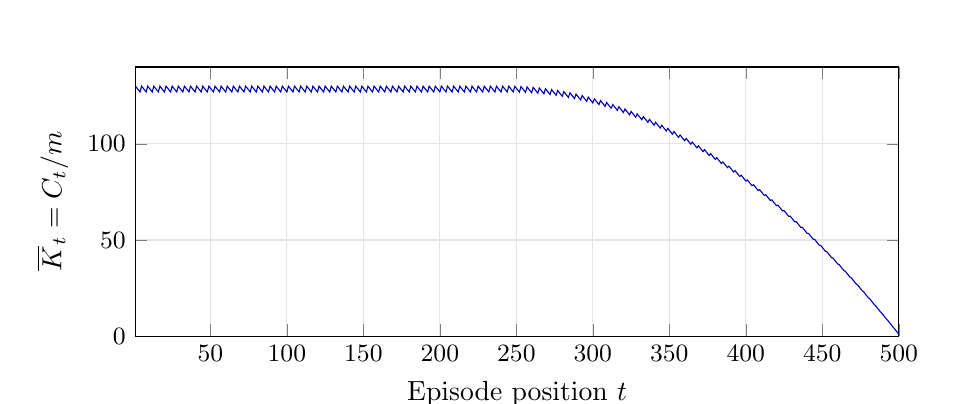
\begin{tikzpicture}\begin{axis}[width=.93\linewidth,height=5cm,xmin=1,xmax=500,ymin=0,ymax=140,xlabel={Episode position $t$},ylabel={$\overline K_t=C_t/m$},grid=major,grid style={gray!20},tick label style={font=\small}]
\addplot[blue!70!black,thin] coordinates {(1,130.00000000)
(2,129.00000000)
(3,128.00000000)
(4,127.00000000)
(5,130.00000000)
(6,129.00000000)
(7,128.00000000)
(8,127.00000000)
(9,130.00000000)
(10,129.00000000)
(11,128.00000000)
(12,127.00000000)
(13,130.00000000)
(14,129.00000000)
(15,128.00000000)
(16,127.00000000)
(17,130.00000000)
(18,129.00000000)
(19,128.00000000)
(20,127.00000000)
(21,130.00000000)
(22,129.00000000)
(23,128.00000000)
(24,127.00000000)
(25,130.00000000)
(26,129.00000000)
(27,128.00000000)
(28,127.00000000)
(29,130.00000000)
(30,129.00000000)
(31,128.00000000)
(32,127.00000000)
(33,130.00000000)
(34,129.00000000)
(35,128.00000000)
(36,127.00000000)
(37,130.00000000)
(38,129.00000000)
(39,128.00000000)
(40,127.00000000)
(41,130.00000000)
(42,129.00000000)
(43,128.00000000)
(44,127.00000000)
(45,130.00000000)
(46,129.00000000)
(47,128.00000000)
(48,127.00000000)
(49,130.00000000)
(50,129.00000000)
(51,128.00000000)
(52,127.00000000)
(53,130.00000000)
(54,129.00000000)
(55,128.00000000)
(56,127.00000000)
(57,130.00000000)
(58,129.00000000)
(59,128.00000000)
(60,127.00000000)
(61,130.00000000)
(62,129.00000000)
(63,128.00000000)
(64,127.00000000)
(65,130.00000000)
(66,129.00000000)
(67,128.00000000)
(68,127.00000000)
(69,130.00000000)
(70,129.00000000)
(71,128.00000000)
(72,127.00000000)
(73,130.00000000)
(74,129.00000000)
(75,128.00000000)
(76,127.00000000)
(77,130.00000000)
(78,129.00000000)
(79,128.00000000)
(80,127.00000000)
(81,130.00000000)
(82,129.00000000)
(83,128.00000000)
(84,127.00000000)
(85,130.00000000)
(86,129.00000000)
(87,128.00000000)
(88,127.00000000)
(89,130.00000000)
(90,129.00000000)
(91,128.00000000)
(92,127.00000000)
(93,130.00000000)
(94,129.00000000)
(95,128.00000000)
(96,127.00000000)
(97,130.00000000)
(98,129.00000000)
(99,128.00000000)
(100,127.00000000)
(101,130.00000000)
(102,129.00000000)
(103,128.00000000)
(104,127.00000000)
(105,130.00000000)
(106,129.00000000)
(107,128.00000000)
(108,127.00000000)
(109,130.00000000)
(110,129.00000000)
(111,128.00000000)
(112,127.00000000)
(113,130.00000000)
(114,129.00000000)
(115,128.00000000)
(116,127.00000000)
(117,130.00000000)
(118,129.00000000)
(119,128.00000000)
(120,127.00000000)
(121,130.00000000)
(122,129.00000000)
(123,128.00000000)
(124,127.00000000)
(125,130.00000000)
(126,129.00000000)
(127,128.00000000)
(128,127.00000000)
(129,130.00000000)
(130,129.00000000)
(131,128.00000000)
(132,127.00000000)
(133,130.00000000)
(134,129.00000000)
(135,128.00000000)
(136,127.00000000)
(137,130.00000000)
(138,129.00000000)
(139,128.00000000)
(140,127.00000000)
(141,130.00000000)
(142,129.00000000)
(143,128.00000000)
(144,127.00000000)
(145,130.00000000)
(146,129.00000000)
(147,128.00000000)
(148,127.00000000)
(149,130.00000000)
(150,129.00000000)
(151,128.00000000)
(152,127.00000000)
(153,130.00000000)
(154,129.00000000)
(155,128.00000000)
(156,127.00000000)
(157,130.00000000)
(158,129.00000000)
(159,128.00000000)
(160,127.00000000)
(161,130.00000000)
(162,129.00000000)
(163,128.00000000)
(164,127.00000000)
(165,130.00000000)
(166,129.00000000)
(167,128.00000000)
(168,127.00000000)
(169,130.00000000)
(170,129.00000000)
(171,128.00000000)
(172,127.00000000)
(173,130.00000000)
(174,129.00000000)
(175,128.00000000)
(176,127.00000000)
(177,130.00000000)
(178,129.00000000)
(179,128.00000000)
(180,127.00000000)
(181,130.00000000)
(182,129.00000000)
(183,128.00000000)
(184,127.00000000)
(185,130.00000000)
(186,129.00000000)
(187,128.00000000)
(188,127.00000000)
(189,130.00000000)
(190,129.00000000)
(191,128.00000000)
(192,127.00000000)
(193,130.00000000)
(194,129.00000000)
(195,128.00000000)
(196,127.00000000)
(197,130.00000000)
(198,129.00000000)
(199,128.00000000)
(200,127.00000000)
(201,130.00000000)
(202,129.00000000)
(203,128.00000000)
(204,127.00000000)
(205,130.00000000)
(206,129.00000000)
(207,128.00000000)
(208,127.00000000)
(209,130.00000000)
(210,129.00000000)
(211,128.00000000)
(212,127.00000000)
(213,130.00000000)
(214,129.00000000)
(215,128.00000000)
(216,127.00000000)
(217,130.00000000)
(218,129.00000000)
(219,128.00000000)
(220,127.00000000)
(221,130.00000000)
(222,129.00000000)
(223,128.00000000)
(224,127.00000000)
(225,130.00000000)
(226,129.00000000)
(227,128.00000000)
(228,127.00000000)
(229,130.00000000)
(230,129.00000000)
(231,128.00000000)
(232,127.00000000)
(233,130.00000000)
(234,129.00000000)
(235,128.00000000)
(236,127.00000000)
(237,130.00000000)
(238,129.00000000)
(239,128.00000000)
(240,127.00000000)
(241,130.00000000)
(242,129.00000000)
(243,128.00000000)
(244,127.00000000)
(245,130.00000000)
(246,129.00000000)
(247,128.00000000)
(248,127.00000000)
(249,129.93750000)
(250,128.93750000)
(251,127.93750000)
(252,126.93750000)
(253,129.81250000)
(254,128.81250000)
(255,127.81250000)
(256,126.81250000)
(257,129.62500000)
(258,128.62500000)
(259,127.62500000)
(260,126.62500000)
(261,129.37500000)
(262,128.37500000)
(263,127.37500000)
(264,126.37500000)
(265,129.06250000)
(266,128.06250000)
(267,127.06250000)
(268,126.06250000)
(269,128.68750000)
(270,127.68750000)
(271,126.68750000)
(272,125.68750000)
(273,128.25000000)
(274,127.25000000)
(275,126.25000000)
(276,125.25000000)
(277,127.75000000)
(278,126.75000000)
(279,125.75000000)
(280,124.75000000)
(281,127.18750000)
(282,126.18750000)
(283,125.18750000)
(284,124.18750000)
(285,126.56250000)
(286,125.56250000)
(287,124.56250000)
(288,123.56250000)
(289,125.87500000)
(290,124.87500000)
(291,123.87500000)
(292,122.87500000)
(293,125.12500000)
(294,124.12500000)
(295,123.12500000)
(296,122.12500000)
(297,124.31250000)
(298,123.31250000)
(299,122.31250000)
(300,121.31250000)
(301,123.43750000)
(302,122.43750000)
(303,121.43750000)
(304,120.43750000)
(305,122.50000000)
(306,121.50000000)
(307,120.50000000)
(308,119.50000000)
(309,121.50000000)
(310,120.50000000)
(311,119.50000000)
(312,118.50000000)
(313,120.43750000)
(314,119.43750000)
(315,118.43750000)
(316,117.43750000)
(317,119.31250000)
(318,118.31250000)
(319,117.31250000)
(320,116.31250000)
(321,118.12500000)
(322,117.12500000)
(323,116.12500000)
(324,115.12500000)
(325,116.87500000)
(326,115.87500000)
(327,114.87500000)
(328,113.87500000)
(329,115.56250000)
(330,114.56250000)
(331,113.56250000)
(332,112.56250000)
(333,114.18750000)
(334,113.18750000)
(335,112.18750000)
(336,111.18750000)
(337,112.75000000)
(338,111.75000000)
(339,110.75000000)
(340,109.75000000)
(341,111.25000000)
(342,110.25000000)
(343,109.25000000)
(344,108.25000000)
(345,109.68750000)
(346,108.68750000)
(347,107.68750000)
(348,106.68750000)
(349,108.06250000)
(350,107.06250000)
(351,106.06250000)
(352,105.06250000)
(353,106.37500000)
(354,105.37500000)
(355,104.37500000)
(356,103.37500000)
(357,104.62500000)
(358,103.62500000)
(359,102.62500000)
(360,101.62500000)
(361,102.81250000)
(362,101.81250000)
(363,100.81250000)
(364,99.81250000)
(365,100.93750000)
(366,99.93750000)
(367,98.93750000)
(368,97.93750000)
(369,99.00000000)
(370,98.00000000)
(371,97.00000000)
(372,96.00000000)
(373,97.00000000)
(374,96.00000000)
(375,95.00000000)
(376,94.00000000)
(377,94.93750000)
(378,93.93750000)
(379,92.93750000)
(380,91.93750000)
(381,92.81250000)
(382,91.81250000)
(383,90.81250000)
(384,89.81250000)
(385,90.62500000)
(386,89.62500000)
(387,88.62500000)
(388,87.62500000)
(389,88.37500000)
(390,87.37500000)
(391,86.37500000)
(392,85.37500000)
(393,86.06250000)
(394,85.06250000)
(395,84.06250000)
(396,83.06250000)
(397,83.68750000)
(398,82.68750000)
(399,81.68750000)
(400,80.68750000)
(401,81.25000000)
(402,80.25000000)
(403,79.25000000)
(404,78.25000000)
(405,78.75000000)
(406,77.75000000)
(407,76.75000000)
(408,75.75000000)
(409,76.18750000)
(410,75.18750000)
(411,74.18750000)
(412,73.18750000)
(413,73.56250000)
(414,72.56250000)
(415,71.56250000)
(416,70.56250000)
(417,70.87500000)
(418,69.87500000)
(419,68.87500000)
(420,67.87500000)
(421,68.12500000)
(422,67.12500000)
(423,66.12500000)
(424,65.12500000)
(425,65.31250000)
(426,64.31250000)
(427,63.31250000)
(428,62.31250000)
(429,62.43750000)
(430,61.43750000)
(431,60.43750000)
(432,59.43750000)
(433,59.50000000)
(434,58.50000000)
(435,57.50000000)
(436,56.50000000)
(437,56.50000000)
(438,55.50000000)
(439,54.50000000)
(440,53.50000000)
(441,53.43750000)
(442,52.43750000)
(443,51.43750000)
(444,50.43750000)
(445,50.31250000)
(446,49.31250000)
(447,48.31250000)
(448,47.31250000)
(449,47.12500000)
(450,46.12500000)
(451,45.12500000)
(452,44.12500000)
(453,43.87500000)
(454,42.87500000)
(455,41.87500000)
(456,40.87500000)
(457,40.56250000)
(458,39.56250000)
(459,38.56250000)
(460,37.56250000)
(461,37.18750000)
(462,36.18750000)
(463,35.18750000)
(464,34.18750000)
(465,33.75000000)
(466,32.75000000)
(467,31.75000000)
(468,30.75000000)
(469,30.25000000)
(470,29.25000000)
(471,28.25000000)
(472,27.25000000)
(473,26.68750000)
(474,25.68750000)
(475,24.68750000)
(476,23.68750000)
(477,23.06250000)
(478,22.06250000)
(479,21.06250000)
(480,20.06250000)
(481,19.37500000)
(482,18.37500000)
(483,17.37500000)
(484,16.37500000)
(485,15.62500000)
(486,14.62500000)
(487,13.62500000)
(488,12.62500000)
(489,11.81250000)
(490,10.81250000)
(491,9.81250000)
(492,8.81250000)
(493,7.93750000)
(494,6.93750000)
(495,5.93750000)
(496,4.93750000)
(497,4.00000000)
(498,3.00000000)
(499,2.00000000)
(500,1.00000000)};
\end{axis}\end{tikzpicture}
\par\medskip
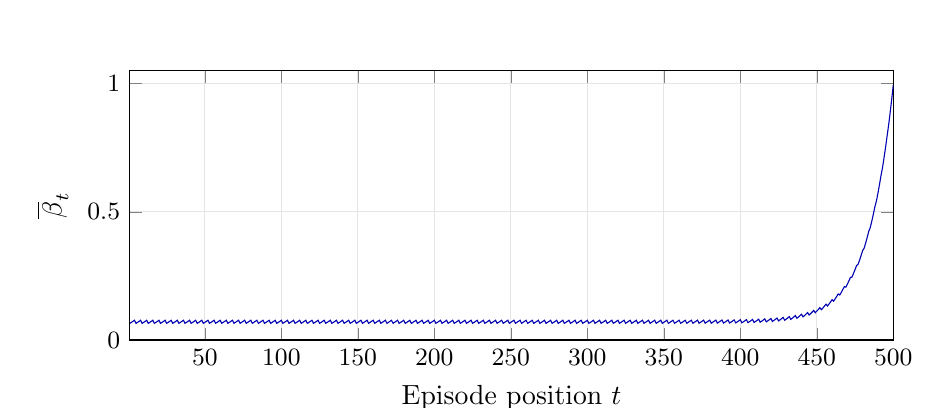
\begin{tikzpicture}\begin{axis}[width=.93\linewidth,height=5cm,xmin=1,xmax=500,ymin=0,ymax=1.05,xlabel={Episode position $t$},ylabel={$\overline\beta_t$},grid=major,grid style={gray!20},tick label style={font=\small}]
\addplot[blue!70!black,thin] coordinates {(1,0.06511164)
(2,0.06888298)
(3,0.07287277)
(4,0.07709364)
(5,0.06511164)
(6,0.06888298)
(7,0.07287277)
(8,0.07709364)
(9,0.06511164)
(10,0.06888298)
(11,0.07287277)
(12,0.07709364)
(13,0.06511164)
(14,0.06888298)
(15,0.07287277)
(16,0.07709364)
(17,0.06511164)
(18,0.06888298)
(19,0.07287277)
(20,0.07709364)
(21,0.06511164)
(22,0.06888298)
(23,0.07287277)
(24,0.07709364)
(25,0.06511164)
(26,0.06888298)
(27,0.07287277)
(28,0.07709364)
(29,0.06511164)
(30,0.06888298)
(31,0.07287277)
(32,0.07709364)
(33,0.06511164)
(34,0.06888298)
(35,0.07287277)
(36,0.07709364)
(37,0.06511164)
(38,0.06888298)
(39,0.07287277)
(40,0.07709364)
(41,0.06511164)
(42,0.06888298)
(43,0.07287277)
(44,0.07709364)
(45,0.06511164)
(46,0.06888298)
(47,0.07287277)
(48,0.07709364)
(49,0.06511164)
(50,0.06888298)
(51,0.07287277)
(52,0.07709364)
(53,0.06511164)
(54,0.06888298)
(55,0.07287277)
(56,0.07709364)
(57,0.06511164)
(58,0.06888298)
(59,0.07287277)
(60,0.07709364)
(61,0.06511164)
(62,0.06888298)
(63,0.07287277)
(64,0.07709364)
(65,0.06511164)
(66,0.06888298)
(67,0.07287277)
(68,0.07709364)
(69,0.06511164)
(70,0.06888298)
(71,0.07287277)
(72,0.07709364)
(73,0.06511164)
(74,0.06888298)
(75,0.07287277)
(76,0.07709364)
(77,0.06511164)
(78,0.06888298)
(79,0.07287277)
(80,0.07709364)
(81,0.06511164)
(82,0.06888298)
(83,0.07287277)
(84,0.07709364)
(85,0.06511164)
(86,0.06888298)
(87,0.07287277)
(88,0.07709364)
(89,0.06511164)
(90,0.06888298)
(91,0.07287277)
(92,0.07709364)
(93,0.06511164)
(94,0.06888298)
(95,0.07287277)
(96,0.07709364)
(97,0.06511164)
(98,0.06888298)
(99,0.07287277)
(100,0.07709364)
(101,0.06511164)
(102,0.06888298)
(103,0.07287277)
(104,0.07709364)
(105,0.06511164)
(106,0.06888298)
(107,0.07287277)
(108,0.07709364)
(109,0.06511164)
(110,0.06888298)
(111,0.07287277)
(112,0.07709364)
(113,0.06511164)
(114,0.06888298)
(115,0.07287277)
(116,0.07709364)
(117,0.06511164)
(118,0.06888298)
(119,0.07287277)
(120,0.07709364)
(121,0.06511164)
(122,0.06888298)
(123,0.07287277)
(124,0.07709364)
(125,0.06511164)
(126,0.06888298)
(127,0.07287277)
(128,0.07709364)
(129,0.06511164)
(130,0.06888298)
(131,0.07287277)
(132,0.07709364)
(133,0.06511164)
(134,0.06888298)
(135,0.07287277)
(136,0.07709364)
(137,0.06511164)
(138,0.06888298)
(139,0.07287277)
(140,0.07709364)
(141,0.06511164)
(142,0.06888298)
(143,0.07287277)
(144,0.07709364)
(145,0.06511164)
(146,0.06888298)
(147,0.07287277)
(148,0.07709364)
(149,0.06511164)
(150,0.06888298)
(151,0.07287277)
(152,0.07709364)
(153,0.06511164)
(154,0.06888298)
(155,0.07287277)
(156,0.07709364)
(157,0.06511164)
(158,0.06888298)
(159,0.07287277)
(160,0.07709364)
(161,0.06511164)
(162,0.06888298)
(163,0.07287277)
(164,0.07709364)
(165,0.06511164)
(166,0.06888298)
(167,0.07287277)
(168,0.07709364)
(169,0.06511164)
(170,0.06888298)
(171,0.07287277)
(172,0.07709364)
(173,0.06511164)
(174,0.06888298)
(175,0.07287277)
(176,0.07709364)
(177,0.06511164)
(178,0.06888298)
(179,0.07287277)
(180,0.07709364)
(181,0.06511164)
(182,0.06888298)
(183,0.07287277)
(184,0.07709364)
(185,0.06511164)
(186,0.06888298)
(187,0.07287277)
(188,0.07709364)
(189,0.06511164)
(190,0.06888298)
(191,0.07287277)
(192,0.07709364)
(193,0.06511164)
(194,0.06888298)
(195,0.07287277)
(196,0.07709364)
(197,0.06511164)
(198,0.06888298)
(199,0.07287277)
(200,0.07709364)
(201,0.06511164)
(202,0.06888298)
(203,0.07287277)
(204,0.07709364)
(205,0.06511164)
(206,0.06888298)
(207,0.07287277)
(208,0.07709364)
(209,0.06511164)
(210,0.06888298)
(211,0.07287277)
(212,0.07709364)
(213,0.06511164)
(214,0.06888298)
(215,0.07287277)
(216,0.07709364)
(217,0.06511164)
(218,0.06888298)
(219,0.07287277)
(220,0.07709364)
(221,0.06511164)
(222,0.06888298)
(223,0.07287277)
(224,0.07709364)
(225,0.06511164)
(226,0.06888298)
(227,0.07287277)
(228,0.07709364)
(229,0.06511164)
(230,0.06888298)
(231,0.07287277)
(232,0.07709364)
(233,0.06511164)
(234,0.06888298)
(235,0.07287277)
(236,0.07709364)
(237,0.06511164)
(238,0.06888298)
(239,0.07287277)
(240,0.07709364)
(241,0.06511164)
(242,0.06888298)
(243,0.07287277)
(244,0.07709364)
(245,0.06511164)
(246,0.06888298)
(247,0.07287277)
(248,0.07709364)
(249,0.06511164)
(250,0.06888298)
(251,0.07287277)
(252,0.07709365)
(253,0.06511165)
(254,0.06888299)
(255,0.07287278)
(256,0.07709365)
(257,0.06511166)
(258,0.06888300)
(259,0.07287279)
(260,0.07709367)
(261,0.06511168)
(262,0.06888302)
(263,0.07287281)
(264,0.07709369)
(265,0.06511170)
(266,0.06888305)
(267,0.07287284)
(268,0.07709372)
(269,0.06511175)
(270,0.06888310)
(271,0.07287289)
(272,0.07709377)
(273,0.06511181)
(274,0.06888316)
(275,0.07287296)
(276,0.07709384)
(277,0.06511190)
(278,0.06888325)
(279,0.07287305)
(280,0.07709395)
(281,0.06511202)
(282,0.06888339)
(283,0.07287319)
(284,0.07709410)
(285,0.06511219)
(286,0.06888357)
(287,0.07287339)
(288,0.07709430)
(289,0.06511243)
(290,0.06888382)
(291,0.07287365)
(292,0.07709458)
(293,0.06511276)
(294,0.06888417)
(295,0.07287402)
(296,0.07709497)
(297,0.06511320)
(298,0.06888464)
(299,0.07287452)
(300,0.07709549)
(301,0.06511380)
(302,0.06888527)
(303,0.07287518)
(304,0.07709620)
(305,0.06511460)
(306,0.06888612)
(307,0.07287608)
(308,0.07709715)
(309,0.06511567)
(310,0.06888725)
(311,0.07287728)
(312,0.07709842)
(313,0.06511710)
(314,0.06888876)
(315,0.07287888)
(316,0.07710011)
(317,0.06511899)
(318,0.06889076)
(319,0.07288099)
(320,0.07710234)
(321,0.06512149)
(322,0.06889340)
(323,0.07288379)
(324,0.07710530)
(325,0.06512478)
(326,0.06889689)
(327,0.07288748)
(328,0.07710921)
(329,0.06512912)
(330,0.06890147)
(331,0.07289233)
(332,0.07711434)
(333,0.06513481)
(334,0.06890749)
(335,0.07289870)
(336,0.07712107)
(337,0.06514226)
(338,0.06891537)
(339,0.07290703)
(340,0.07712989)
(341,0.06515199)
(342,0.06892567)
(343,0.07291793)
(344,0.07714142)
(345,0.06516470)
(346,0.06893911)
(347,0.07293215)
(348,0.07715646)
(349,0.06518125)
(350,0.06895662)
(351,0.07295067)
(352,0.07717606)
(353,0.06520277)
(354,0.06897940)
(355,0.07297476)
(356,0.07720155)
(357,0.06523074)
(358,0.06900898)
(359,0.07300606)
(360,0.07723466)
(361,0.06526702)
(362,0.06904736)
(363,0.07304666)
(364,0.07727761)
(365,0.06531403)
(366,0.06909709)
(367,0.07309928)
(368,0.07733327)
(369,0.06537487)
(370,0.06916146)
(371,0.07316738)
(372,0.07740532)
(373,0.06545355)
(374,0.06924470)
(375,0.07325543)
(376,0.07749847)
(377,0.06555518)
(378,0.06935222)
(379,0.07336918)
(380,0.07761881)
(381,0.06568634)
(382,0.06949097)
(383,0.07351597)
(384,0.07777410)
(385,0.06585547)
(386,0.06966989)
(387,0.07370525)
(388,0.07797435)
(389,0.06607336)
(390,0.06990041)
(391,0.07394912)
(392,0.07823235)
(393,0.06635388)
(394,0.07019718)
(395,0.07426308)
(396,0.07856449)
(397,0.06671476)
(398,0.07057896)
(399,0.07466698)
(400,0.07899178)
(401,0.06717869)
(402,0.07106976)
(403,0.07518621)
(404,0.07954108)
(405,0.06777471)
(406,0.07170031)
(407,0.07585327)
(408,0.08024678)
(409,0.06853996)
(410,0.07250987)
(411,0.07670973)
(412,0.08115285)
(413,0.06952188)
(414,0.07354867)
(415,0.07780870)
(416,0.08231547)
(417,0.07078113)
(418,0.07488086)
(419,0.07921804)
(420,0.08380645)
(421,0.07239515)
(422,0.07658836)
(423,0.08102445)
(424,0.08571748)
(425,0.07446282)
(426,0.07877579)
(427,0.08333858)
(428,0.08816565)
(429,0.07711034)
(430,0.08157666)
(431,0.08630168)
(432,0.09130038)
(433,0.08049873)
(434,0.08516131)
(435,0.09009396)
(436,0.09531231)
(437,0.08483334)
(438,0.08974699)
(439,0.09494524)
(440,0.10044458)
(441,0.09037600)
(442,0.09561068)
(443,0.10114856)
(444,0.10700721)
(445,0.09746043)
(446,0.10310545)
(447,0.10907744)
(448,0.11539534)
(449,0.10651189)
(450,0.11268118)
(451,0.11920781)
(452,0.12611247)
(453,0.11807208)
(454,0.12491095)
(455,0.13214594)
(456,0.13979999)
(457,0.13283087)
(458,0.14052459)
(459,0.14866394)
(460,0.15727473)
(461,0.15166658)
(462,0.16045128)
(463,0.16974481)
(464,0.17957663)
(465,0.17569715)
(466,0.18587374)
(467,0.19663976)
(468,0.20802937)
(469,0.20634519)
(470,0.21829695)
(471,0.23094096)
(472,0.24431734)
(473,0.24542053)
(474,0.25963558)
(475,0.27467398)
(476,0.29058342)
(477,0.29522510)
(478,0.31232488)
(479,0.33041511)
(480,0.34955315)
(481,0.35868603)
(482,0.37946155)
(483,0.40144041)
(484,0.42469232)
(485,0.43952466)
(486,0.46498245)
(487,0.49191478)
(488,0.52040707)
(489,0.54247097)
(490,0.57389153)
(491,0.60713201)
(492,0.64229781)
(493,0.67353572)
(494,0.71254771)
(495,0.75381931)
(496,0.79748142)
(497,0.84035568)
(498,0.88903007)
(499,0.94052375)
(500,0.99500000)};
\end{axis}\end{tikzpicture}
\caption{Average observed reward support (top) and average endpoint-error sensitivity (bottom) over 64 episodes. Small oscillations reflect the four residue classes of the rollout phase. Endpoint sensitivity rises sharply near the episode boundary. The bottom curve is a coefficient, not measured critic error.}\label{fig:support}
\end{figure}

\subsection{Why the support distribution, rather than its mean alone, matters}
Define the empirical support-length distribution
\begin{equation}
 p_t(k)=\frac1m\sum_{j=1}^{m}\ind\{K_{j,t}=k\}.
\end{equation}
Then $C_t/m=\E_{p_t}[K]$, whereas
$\bar\beta_t=\gamma\E_{p_t}[q^{K-1}]$.
For two length sets $(1,5)$ and $(3,3)$, both have cumulative support 6, but
\begin{equation}
 \frac\gamma2(1+q^4)-\gamma q^2
 =\frac\gamma2(1-q^2)^2>0.
\end{equation}
Consequently, replacing every $K$ with $\bar K_t$ does not give the correct average
sensitivity. Indeed, convexity gives
\begin{equation}
 \bar\beta_t\ge\gamma q^{\bar K_t-1}.
\end{equation}
Short fragments can dominate endpoint sensitivity even when average reward
support is large. In particular, the first position's average support 130 does
not mean it behaves like a single 130-step estimator.

\subsection{A uniform bound on all critic errors}
If $|e(s)|\le\varepsilon$, Equation~\eqref{eq:bias} implies
\begin{equation}
 |b_K(s)|\le\alpha_K\varepsilon,
\end{equation}
where
\begin{align}\label{eq:alpha}
 \alpha_K
 &=\gamma(1-\lambda)\frac{1-q^{K-1}}{1-q}+\gamma q^{K-1}\nonumber\\
 &=\frac{\gamma(1-\lambda)}{1-q}
 +\frac{\gamma\lambda(1-\gamma)}{1-q}q^{K-1}.
\end{align}
For the example parameters, $\alpha_1=0.995$ and
$\alpha_\infty\simeq0.90868$. Increasing $K$ reduces this uniform bound, but it does
not eliminate intermediate-value dependence when $\lambda<1$.
If $e(s)=c$ is constant across all visited states, the target bias is exactly
$\alpha_Kc$; if $e=0$, the target bias is zero for every support length.
At $\lambda=1$, $\alpha_K=\gamma^K$; at $\lambda=0$, $\alpha_K=\gamma$ for every $K$.
These cases distinguish endpoint-specific sensitivity from the total influence
of a critic whose errors extend across the entire trajectory.

\subsection{From target error to the critic update}
For one sample under a squared loss,
\begin{equation}
 \ell_t=\tfrac12(V_\phi(s_t)-Y_t)^2,\qquad
 \frac{\partial\ell_t}{\partial V_\phi(s_t)}=V_\phi(s_t)-Y_t.
\end{equation}
Holding the current network fixed, a target perturbation produces
\begin{equation}
 \Delta\nabla_\phi\ell_t=-\Delta Y_t\,\nabla_\phi V_\phi(s_t).
\end{equation}
A persistently shifted target repeatedly pushes the fitted value in that direction.
Shared network parameters also couple updates at different states. This equation
describes the local squared-loss update; value clipping or other optimization
modifications can alter the realized gradient.

\section{Sample count, coverage, and the remaining error}
\subsection{More episodes versus longer reward support}
For $m$ independent, identically distributed targets at the same state, the sample
mean estimator satisfies
\begin{equation}
 \E[(\hat V(s)-V^\pi(s))^2]=b_K(s)^2+
 \frac{\Var(Y^{(K)}\mid s)}{m}.
\end{equation}
For independent but nonidentically distributed targets, the corresponding terms
are the squared mean bias and $m^{-2}\sum_j\Var(Y_j\mid s)$; correlated targets
also add covariance terms. Increasing $m$ reduces sampling noise under the stated
independence conditions. It does not automatically remove a systematic target
bias. Increasing $K$ changes the target itself, including both bias and variance.
For the final position, increasing $m$ changes $C_M=m$ but leaves
$\bar K_M=1$ and $\bar\beta_M=\gamma$ unchanged.

A useful supplementary statistic is the sum of reward coefficients:
\begin{equation}
 W_t=\sum_{j=1}^{m}\frac{1-q^{K_{j,t}}}{1-q},\qquad 0<q<1.
\end{equation}
$W_t$ measures total coefficient weight, not an effective independent sample size.
Neither $C_t$ nor $W_t$ alone specifies the learned critic's mean squared error.

\subsection{Why extending episodes can improve endpoint values}
Consider a deterministic chain $s_1\to\cdots\to s_M\to s_{M+1}$, where training
always resets at $s_{M+1}$. Correct bootstrap retains
$Y_M=r_M+\gamma V_{\rm old}(s_{M+1})$, but there is no observed outgoing transition
from $s_{M+1}$ in this dataset. If all observed Bellman equations are satisfied
and the boundary value has error $c$, subtracting the true Bellman equations gives
\begin{equation}
 e(s_t)=\gamma e(s_{t+1})
       =\boxed{\gamma^{M-t+1}c}.
\end{equation}
Thus small Bellman residuals on the observed chain do not determine the unknown
boundary value. Extending episodes makes previously unobserved outgoing
transitions available and moves the unconstrained boundary farther away.
States already covered elsewhere can share these constraints through learning;
what matters is state-transition coverage, not the timestep label by itself.

A rollout boundary is different: the next rollout normally resumes the same
episode, so the outgoing data are eventually collected. It limits the current
GAE fragment without necessarily creating a persistent coverage gap. An episode
reset removes the continuation unless other trajectories visit the relevant states.

\section{Implications for the controlled experiment}
The direct, quantifiable effect is:
\begin{quote}
Late-episode targets have less observed reward support and greater sensitivity
to their final value prediction. Correct bootstrap supplies that prediction but
does not supply the missing realized rewards. Longer episodes can both extend
some fragments and train the predictions on newly observed continuation states.
\end{quote}
The following measurements separate these mechanisms:
\begin{enumerate}
\item Record $K_{j,t}$, $C_t$, and $p_t(k)$ by episode position, together with
$\bar\beta_t$. These are sampling-geometry quantities, not critic-error estimates.
\item Freeze a policy, critic, and normalization statistics; use common long
trajectories to compare targets constructed with different rollout/reset cuts.
Estimate reference values from independent continuations where feasible.
This separates estimator differences from policy changes during training.
\item Measure target error and critic error by position, as well as current,
intermediate, and endpoint prediction errors. A larger $\bar\beta_t$ matters
most where endpoint errors are substantial or systematically signed.
\item Compare training runs with the same physical timestep, reference prefix,
reward definition, total interaction budget, and correct timeout bootstrap.
Longer episodes change the state distribution: the first $H$ steps occupy a
fraction $H/M$ of samples when $H\le M$, which should be reported.
\end{enumerate}

At fixed rollout length, increasing $M$ does not remove rollout boundaries. For
example, in the first episode with $N=256$, position 500 has support 1 when
$M=500$, but support 13 when $M\ge512$, because the next rollout boundary is 512.
Further extension can improve learned continuation values even when it does not
increase that particular sample's immediate support.

For $E$ synchronized environments with identical episode lengths and phases,
all environments have the same $K_{j,t}$. Pooling $m$ episodes \emph{per environment}
multiplies $C_t$ by $E$ but does not change $\bar K_t$ or $\bar\beta_t$.
Variable episode lengths and early failures require the actual cumulative start
index in Equation~\eqref{eq:K}; the fixed-length periodic formulas no longer apply.

This document assumes the timeout semantics described in~\cite{timelimits}:
artificial episode boundaries retain final-state bootstrap, whereas genuine
terminal states have zero continuation value. It makes no claim that a particular
backend currently enforces these semantics; they are the stipulated conditions of
this analysis. All numerical tables use $M=500$ as a mathematical example, not as
a measurement of the actual simulator horizon.

\appendix
\section{Reproducing the counts and sensitivity coefficients}
The following Python fragment uses only the standard library. It verifies the
full-period closed forms against enumeration and prints the values used above.
\begin{verbatim}
from math import gcd
M, N, m = 500, 256, 64
gamma, lam = 0.995, 0.95
q = gamma * lam
d, L = gcd(M, N), N // gcd(M, N)
for t in range(1, M + 1):
    R = M - t + 1
    K = [min(R, N - ((j*M + t - 1) % N))
         for j in range(m)]
    a = (t - 1) % d
    c = d - a
    h = min(L, max(0, (R-c)//d + 1))
    S = h*c + d*h*(h-1)//2 + (L-h)*R
    beta = gamma/L * (
        q**(c-1)*(1-q**(d*h))/(1-q**d)
        + (L-h)*q**(R-1))
    assert sum(K) == S  # here m == L
    measured = sum(gamma*q**(k-1) for k in K)/m
    assert abs(measured-beta) < 1e-12
    if t in [1, 100, 256, 257, 400, 450, 499, 500]:
        print(t, sum(K), sum(K)/m, measured)
\end{verbatim}

\begin{thebibliography}{9}
\bibitem{gae}
J. Schulman, P. Moritz, S. Levine, M. Jordan, and P. Abbeel.
\emph{High-Dimensional Continuous Control Using Generalized Advantage Estimation}.
ICLR, 2016. \href{https://arxiv.org/abs/1506.02438}{arXiv:1506.02438}.
\bibitem{timelimits}
F. Pardo, A. Tavakoli, V. Levdik, and P. Kormushev.
\emph{Time Limits in Reinforcement Learning}. ICML, PMLR 80:4045--4054, 2018.
\href{https://proceedings.mlr.press/v80/pardo18a.html}{Paper and proceedings}.
\end{thebibliography}
\end{document}
